\subsection{Umfrage}
\label{ssec:konzept:client:umfrage}
Wie in Abbildung~\vref{fig:MockUmfrageTeilnehmer} dargestellt, wird der Teilnehmer auf die zuvor angegebene Umfrage geleitet.
Die Fragen werden dabei jeweils in einer eigenen Karte dargestellt.
Durch Drücken eines Knopfes soll der Teilnehmer zur nächsten Frage gelangen.
Gleichzeitig soll dem Benutzer sein Fortschritt verdeutlicht werden, um die Dauer der Umfrage abschätzen zu können.
Die Abgabe der Umfrage erfolgt identisch zum Fragenwechsel.
Der Teilnehmer soll dabei Feedback erhalten, ob seine Teilnahme erfolgreich war.

Durch diesen Vorgang sollen die Anforderungen~\hyperref[Anf:A14]{A14}, die anonyme Teilnahme, sowie \hyperref[Anf:15]{A15}, die einfache Teilnahme an einer Umfrage, erfüllt werden.

\begin{figure}[H]
	\centering
	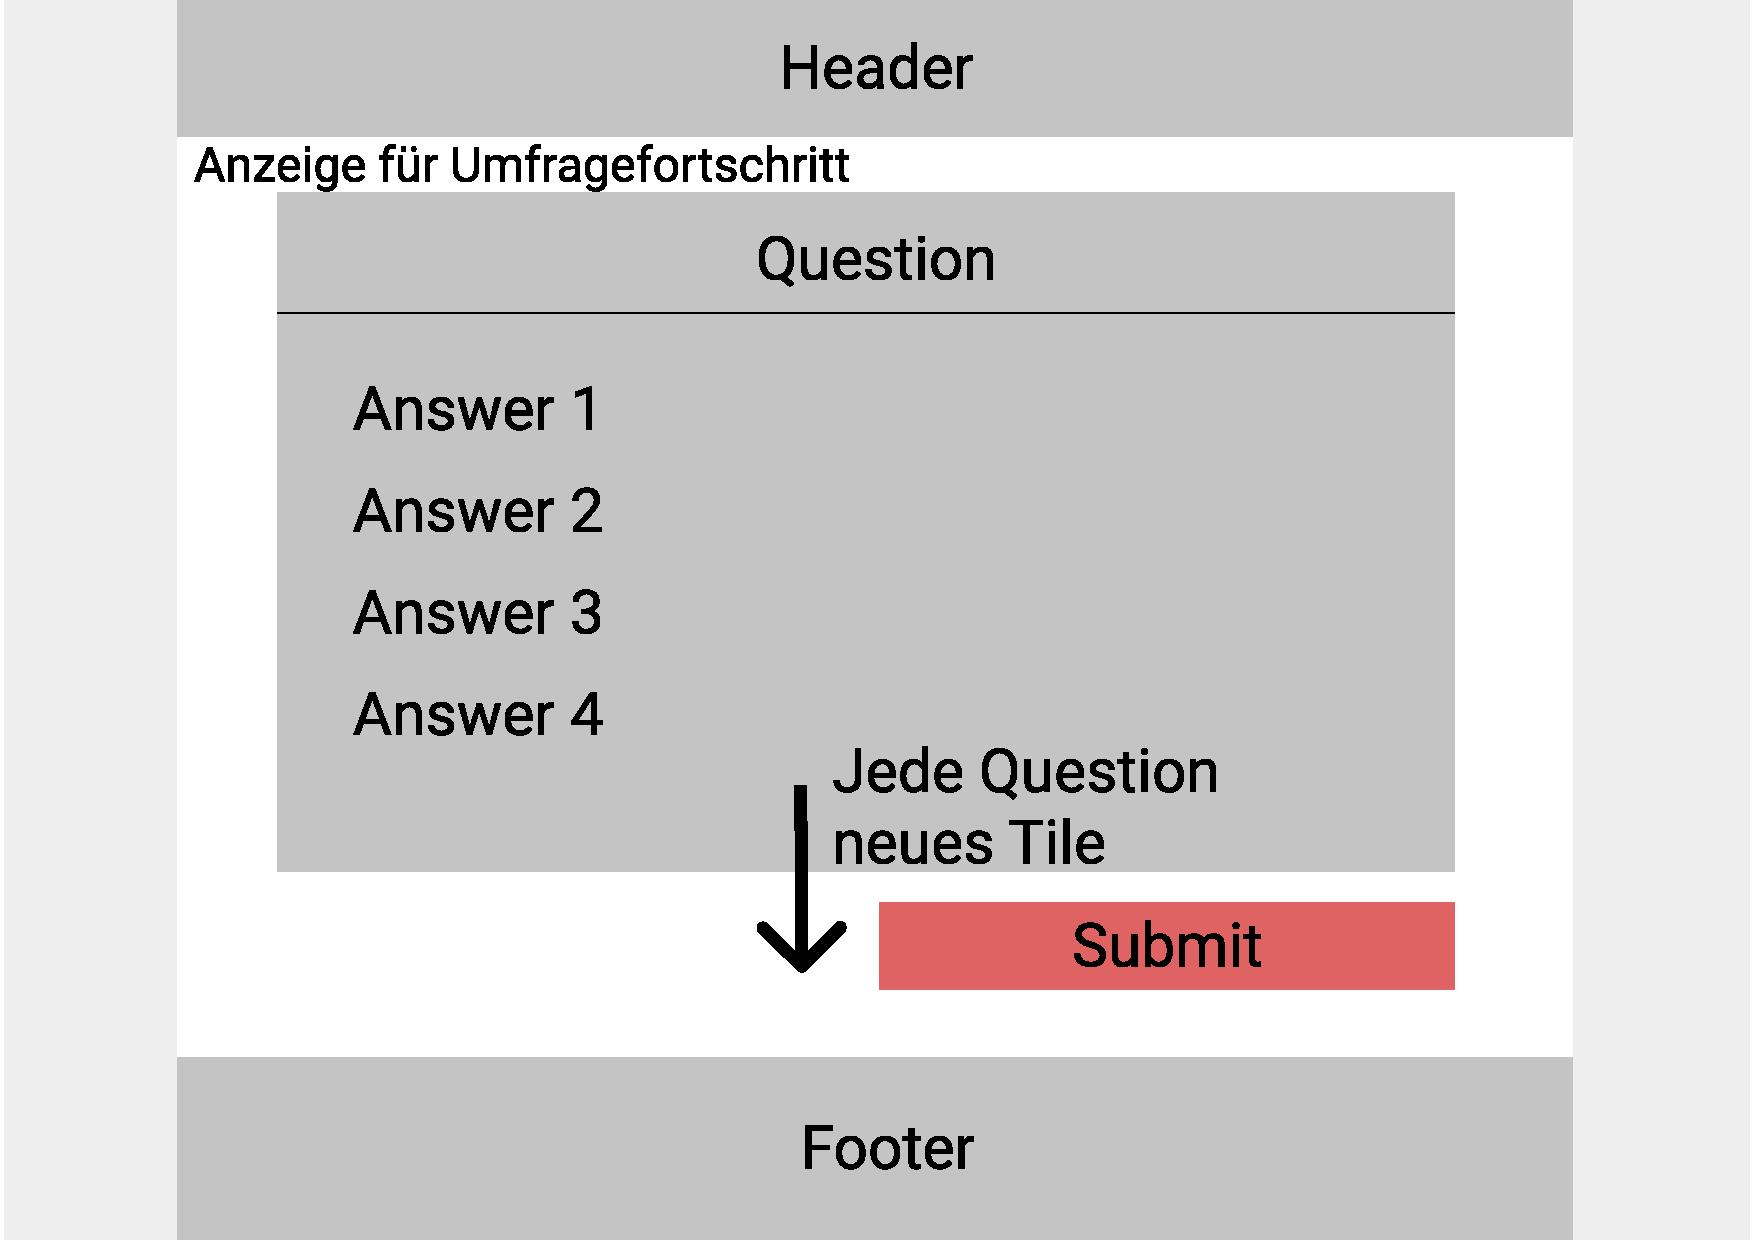
\includegraphics[width=0.7\textwidth]{img/konzeption/client/umfrage_teilnehmer}
	\captionsetup{justification=centering, format=plain}
	\caption[Mock-Up der Teilnahmeseite]{Mock-Up der Teilnahmeseite\\\figma}
	\label{fig:MockUmfrageTeilnehmer}
\end{figure}
